\chapter{Sprawdzenie mo�liwo�� sterowania i pomiaru oraz wyznaczenie punktu pracy}

\section{Przyk�adowe sterowanie wraz z odczytem pomiar�w}

Podczas testu b�dziemy zmienia� sygna�y steruj�ce w nast�puj�cy spos�b:

\begin{align*} 
G1 = 0 \land G2 = 0 & \textrm{, dla } k \in <0, 10) \\ 
G1 = 30 \land G2 = 0 & \textrm{, dla } k \in <10, 30) \\
G1 = 0 \land G2 = 0 & \textrm{, dla } k \in <30, 50) \\
G1 = 0 \land G2 = 40 & \textrm{, dla } k \in <50, 70) \\
G1 = 40 \land G2 = 40 & \textrm{, dla } k \geqslant 70
\end{align*}

\begin{figure}[h!b]
	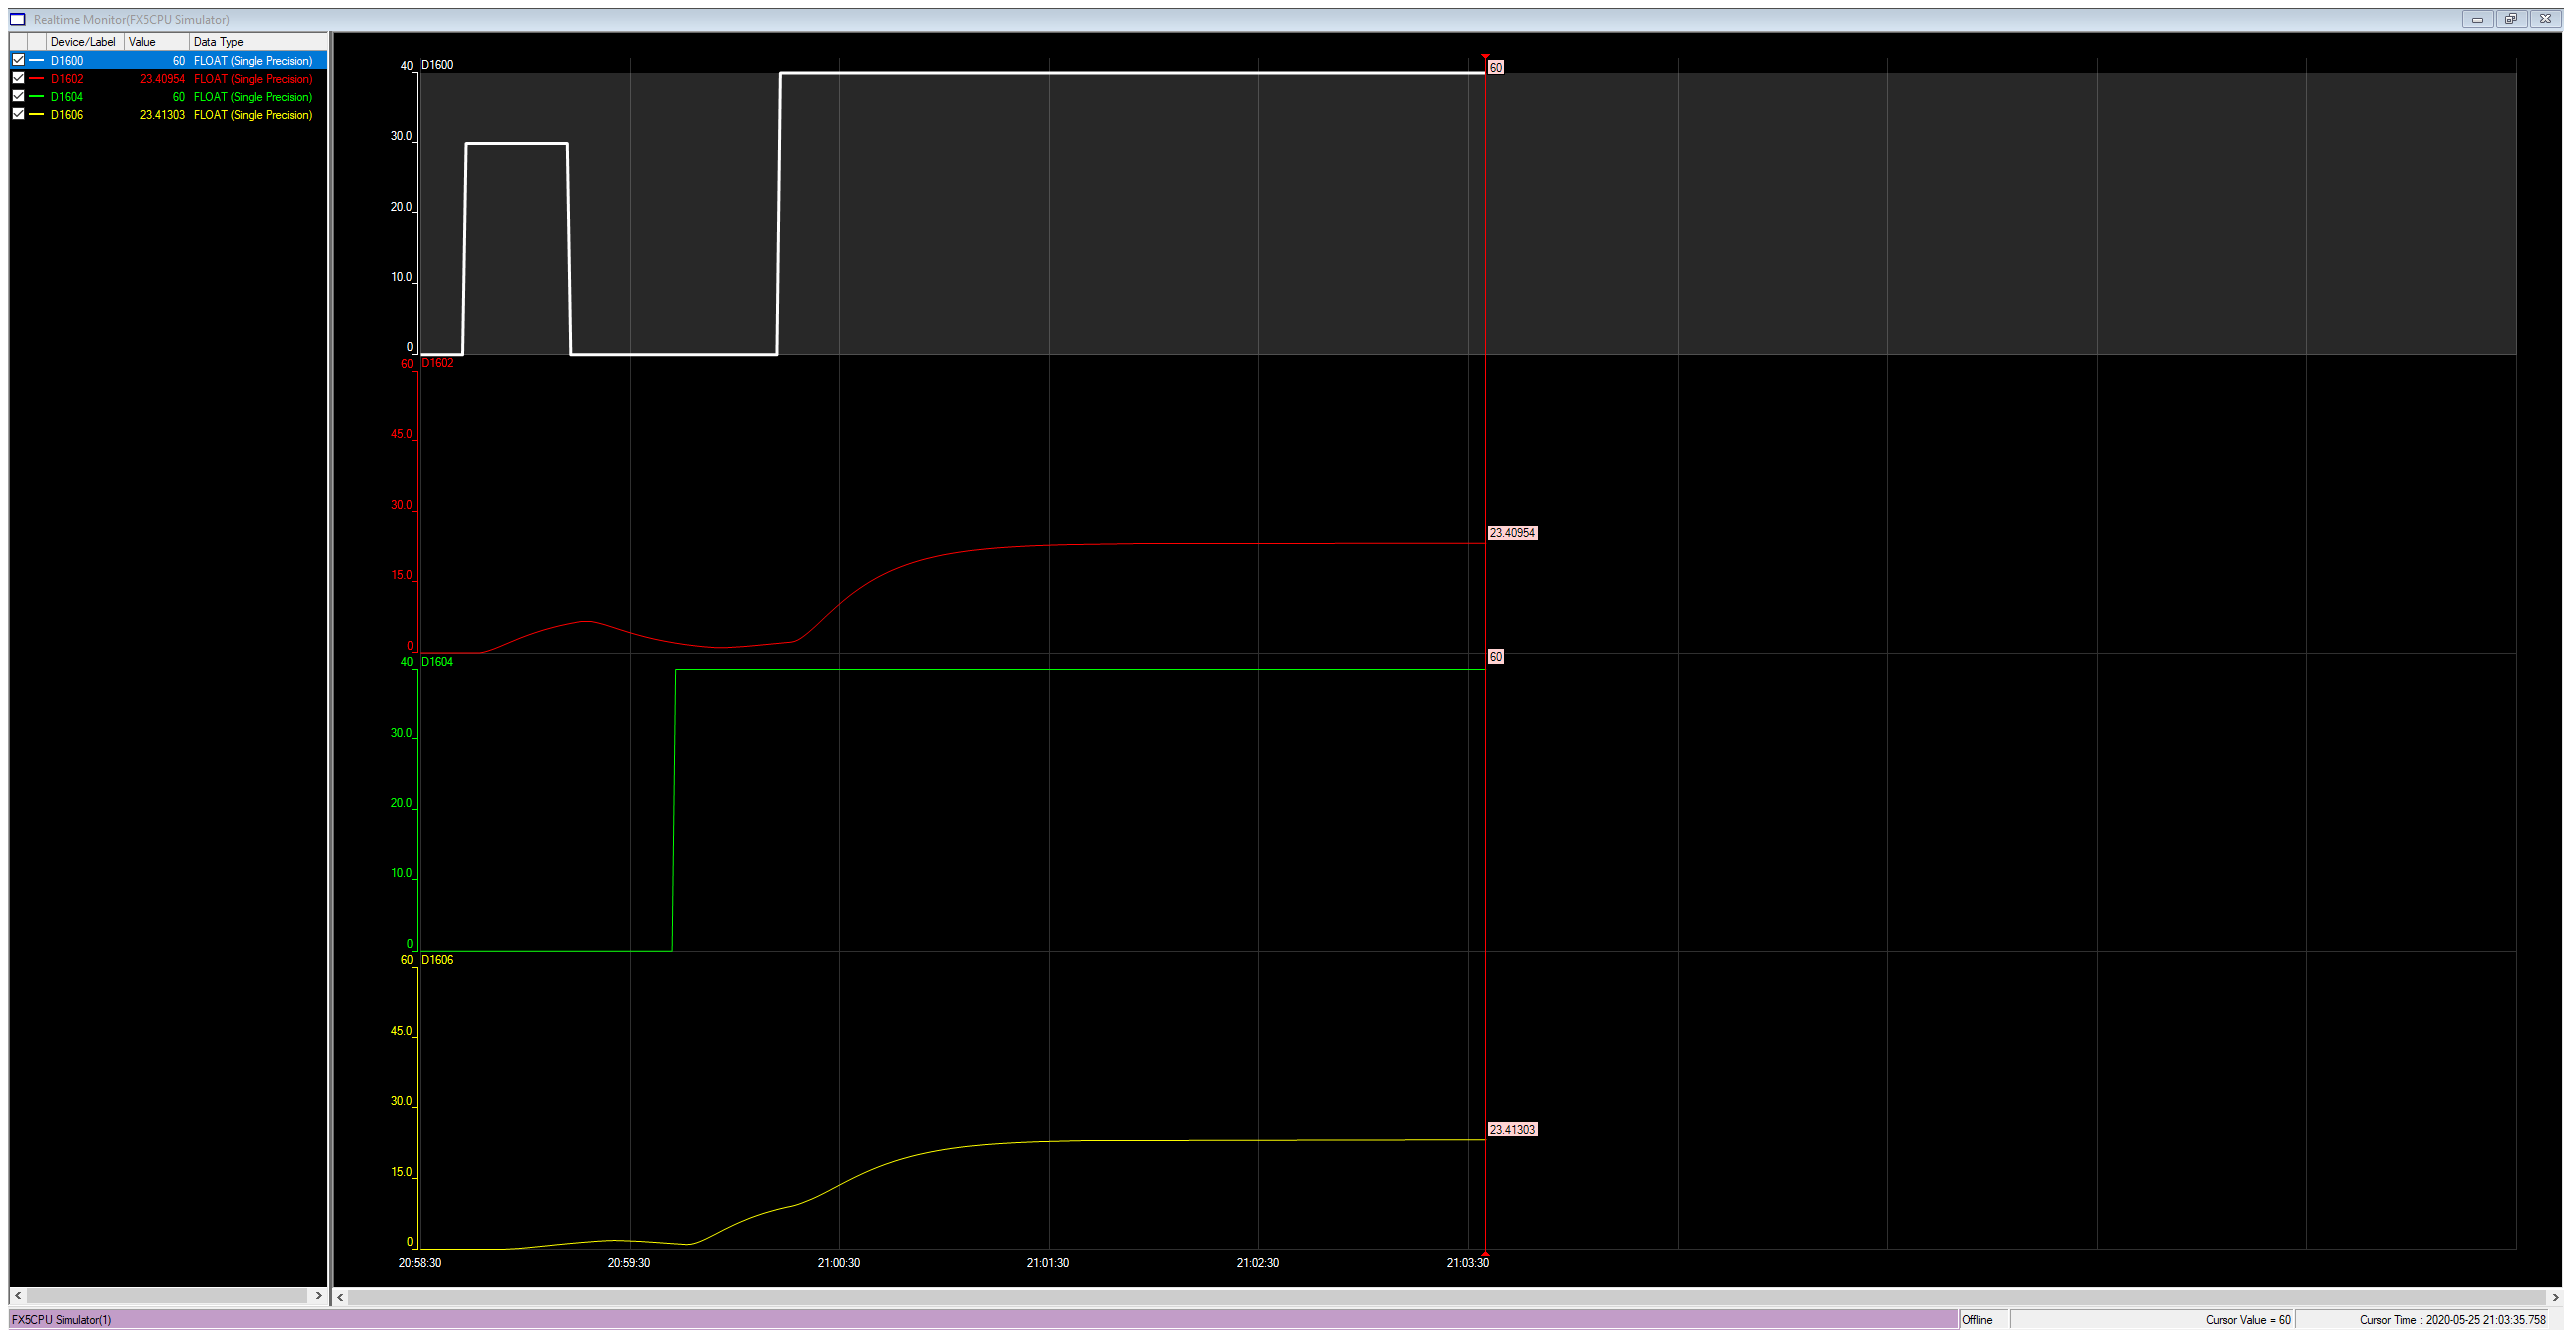
\includegraphics[clip, trim = 0 0 950 0, width=\textwidth, center]{rysunki/COMMUNICATION_CHECK.png}
	\caption{Sprawdzenie mo�liwo�� sterowania i pomiaru w komunikacji ze stanowiskiem - Sygna�y od g�ry: $G1$, $T1$, $G2$, $T3$}
	\label{communication_check}
\end{figure}

Na rys. \ref{communication_check} przedstawiono wyniki przeprowadzonej symulacji. Jak widzimy, zmiany mocy grza�ek $G1$ i $G2$ wp�ywaj� na zmian� mierzonych temperatur $T1$ i $T3$. Oznacza to, mamy mo�liwo�� sterowania i pomiaru w komunikacji ze stanowiskiem.

\section{Punkt pracy}

Zadany punkt pracy: $G1 = \num{28}$, $G2 = \num{33}$. Wyniki symulacji dla tego punktu pracy przedstawiono na rys.~\ref{punkt_pracy}.

\begin{figure}[h!b]
	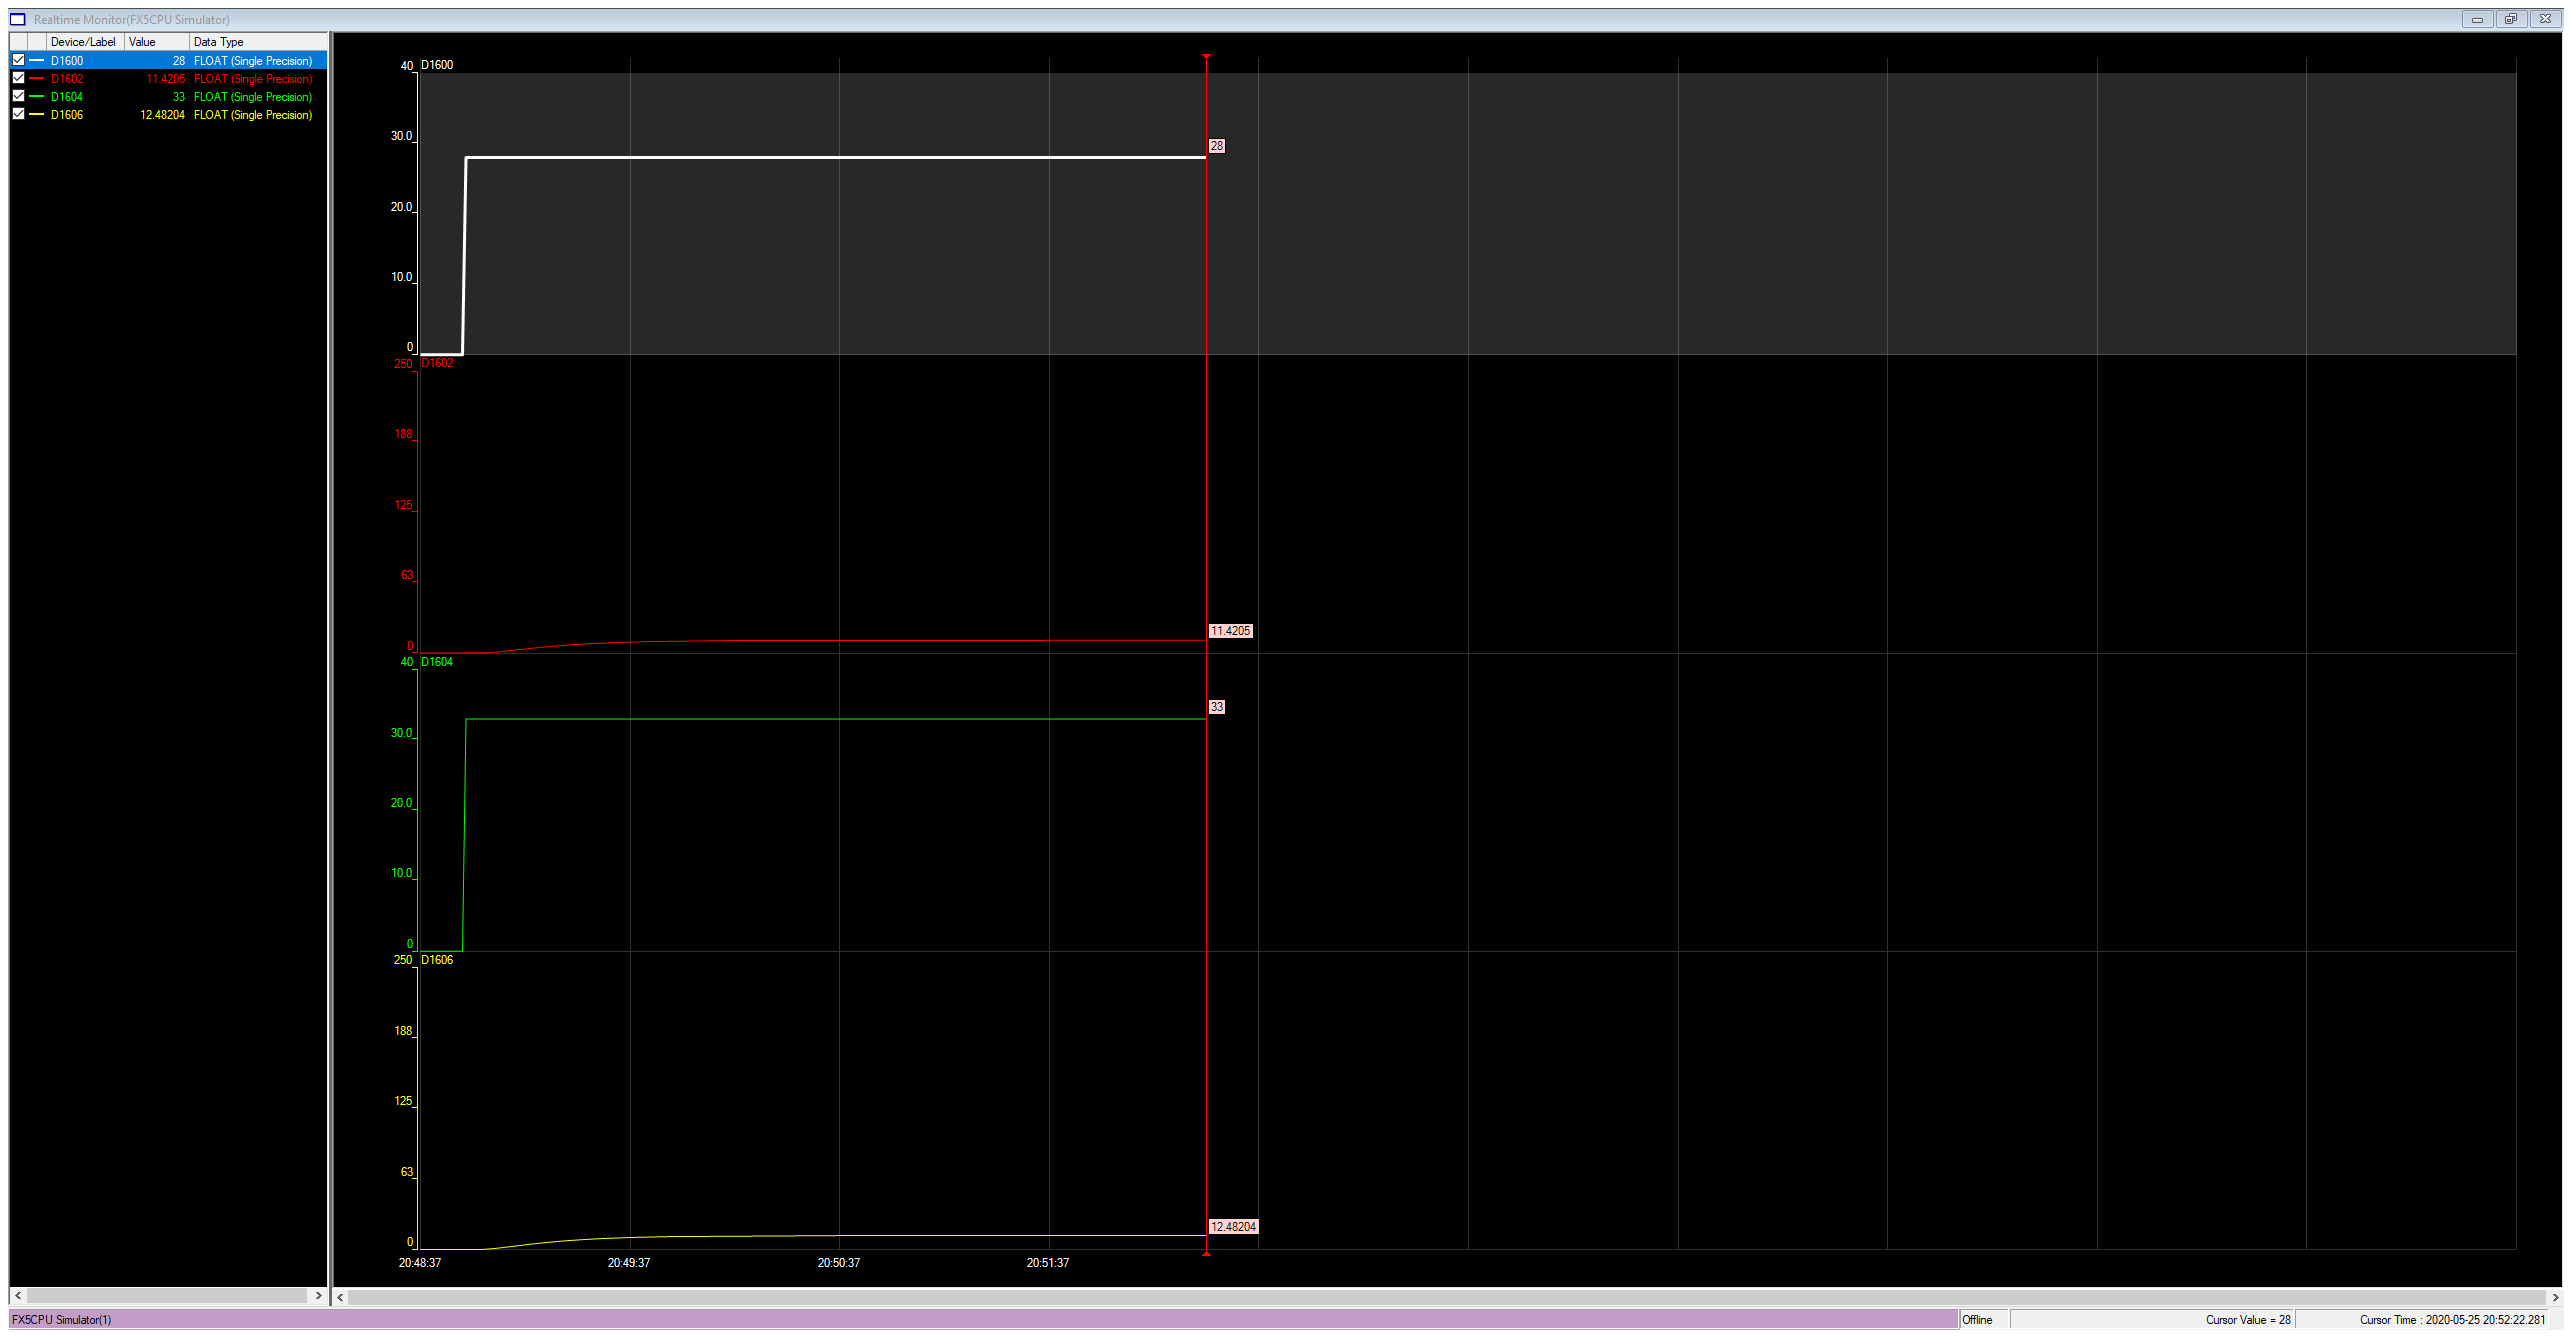
\includegraphics[clip, trim = 0 0 950 0, width=\textwidth, center]{rysunki/PUNKT_PRACY.png}
	\caption{Punkt pracy - Sygna�y od g�ry: $G1$, $T1$, $G2$, $T3$}
	\label{punkt_pracy}
\end{figure}

Dla powy�szego punktu pracy pomiary z czujnik�w wynosz�: $T1 = \num{11.4205}$, $T3 = \num{12.48204}$.